% Options for packages loaded elsewhere
\PassOptionsToPackage{unicode}{hyperref}
\PassOptionsToPackage{hyphens}{url}
%
\documentclass[
  11pt,
  letterpaper,
  DIV=11,
  numbers=noendperiod,
  twoside]{scrartcl}

\usepackage{amsmath,amssymb}
\usepackage{setspace}
\usepackage{iftex}
\ifPDFTeX
  \usepackage[T1]{fontenc}
  \usepackage[utf8]{inputenc}
  \usepackage{textcomp} % provide euro and other symbols
\else % if luatex or xetex
  \usepackage{unicode-math}
  \defaultfontfeatures{Scale=MatchLowercase}
  \defaultfontfeatures[\rmfamily]{Ligatures=TeX,Scale=1}
\fi
\usepackage{lmodern}
\ifPDFTeX\else  
    % xetex/luatex font selection
    \setmainfont[ItalicFont=EB Garamond Italic,BoldFont=EB Garamond
Bold]{EB Garamond Math}
    \setsansfont[]{EB Garamond}
  \setmathfont[]{Garamond-Math}
\fi
% Use upquote if available, for straight quotes in verbatim environments
\IfFileExists{upquote.sty}{\usepackage{upquote}}{}
\IfFileExists{microtype.sty}{% use microtype if available
  \usepackage[]{microtype}
  \UseMicrotypeSet[protrusion]{basicmath} % disable protrusion for tt fonts
}{}
\usepackage{xcolor}
\usepackage[left=1.1in, right=1in, top=0.8in, bottom=0.8in,
paperheight=9.5in, paperwidth=7in, includemp=TRUE, marginparwidth=0in,
marginparsep=0in]{geometry}
\setlength{\emergencystretch}{3em} % prevent overfull lines
\setcounter{secnumdepth}{3}
% Make \paragraph and \subparagraph free-standing
\makeatletter
\ifx\paragraph\undefined\else
  \let\oldparagraph\paragraph
  \renewcommand{\paragraph}{
    \@ifstar
      \xxxParagraphStar
      \xxxParagraphNoStar
  }
  \newcommand{\xxxParagraphStar}[1]{\oldparagraph*{#1}\mbox{}}
  \newcommand{\xxxParagraphNoStar}[1]{\oldparagraph{#1}\mbox{}}
\fi
\ifx\subparagraph\undefined\else
  \let\oldsubparagraph\subparagraph
  \renewcommand{\subparagraph}{
    \@ifstar
      \xxxSubParagraphStar
      \xxxSubParagraphNoStar
  }
  \newcommand{\xxxSubParagraphStar}[1]{\oldsubparagraph*{#1}\mbox{}}
  \newcommand{\xxxSubParagraphNoStar}[1]{\oldsubparagraph{#1}\mbox{}}
\fi
\makeatother


\providecommand{\tightlist}{%
  \setlength{\itemsep}{0pt}\setlength{\parskip}{0pt}}\usepackage{longtable,booktabs,array}
\usepackage{calc} % for calculating minipage widths
% Correct order of tables after \paragraph or \subparagraph
\usepackage{etoolbox}
\makeatletter
\patchcmd\longtable{\par}{\if@noskipsec\mbox{}\fi\par}{}{}
\makeatother
% Allow footnotes in longtable head/foot
\IfFileExists{footnotehyper.sty}{\usepackage{footnotehyper}}{\usepackage{footnote}}
\makesavenoteenv{longtable}
\usepackage{graphicx}
\makeatletter
\newsavebox\pandoc@box
\newcommand*\pandocbounded[1]{% scales image to fit in text height/width
  \sbox\pandoc@box{#1}%
  \Gscale@div\@tempa{\textheight}{\dimexpr\ht\pandoc@box+\dp\pandoc@box\relax}%
  \Gscale@div\@tempb{\linewidth}{\wd\pandoc@box}%
  \ifdim\@tempb\p@<\@tempa\p@\let\@tempa\@tempb\fi% select the smaller of both
  \ifdim\@tempa\p@<\p@\scalebox{\@tempa}{\usebox\pandoc@box}%
  \else\usebox{\pandoc@box}%
  \fi%
}
% Set default figure placement to htbp
\def\fps@figure{htbp}
\makeatother
% definitions for citeproc citations
\NewDocumentCommand\citeproctext{}{}
\NewDocumentCommand\citeproc{mm}{%
  \begingroup\def\citeproctext{#2}\cite{#1}\endgroup}
\makeatletter
 % allow citations to break across lines
 \let\@cite@ofmt\@firstofone
 % avoid brackets around text for \cite:
 \def\@biblabel#1{}
 \def\@cite#1#2{{#1\if@tempswa , #2\fi}}
\makeatother
\newlength{\cslhangindent}
\setlength{\cslhangindent}{1.5em}
\newlength{\csllabelwidth}
\setlength{\csllabelwidth}{3em}
\newenvironment{CSLReferences}[2] % #1 hanging-indent, #2 entry-spacing
 {\begin{list}{}{%
  \setlength{\itemindent}{0pt}
  \setlength{\leftmargin}{0pt}
  \setlength{\parsep}{0pt}
  % turn on hanging indent if param 1 is 1
  \ifodd #1
   \setlength{\leftmargin}{\cslhangindent}
   \setlength{\itemindent}{-1\cslhangindent}
  \fi
  % set entry spacing
  \setlength{\itemsep}{#2\baselineskip}}}
 {\end{list}}
\usepackage{calc}
\newcommand{\CSLBlock}[1]{\hfill\break\parbox[t]{\linewidth}{\strut\ignorespaces#1\strut}}
\newcommand{\CSLLeftMargin}[1]{\parbox[t]{\csllabelwidth}{\strut#1\strut}}
\newcommand{\CSLRightInline}[1]{\parbox[t]{\linewidth - \csllabelwidth}{\strut#1\strut}}
\newcommand{\CSLIndent}[1]{\hspace{\cslhangindent}#1}

\setlength\heavyrulewidth{0ex}
\setlength\lightrulewidth{0ex}
\usepackage[automark]{scrlayer-scrpage}
\clearpairofpagestyles
\cehead{
  Brian Weatherson
  }
\cohead{
  Memory, Belief and Time
  }
\ohead{\bfseries \pagemark}
\cfoot{}
\makeatletter
\newcommand*\NoIndentAfterEnv[1]{%
  \AfterEndEnvironment{#1}{\par\@afterindentfalse\@afterheading}}
\makeatother
\NoIndentAfterEnv{itemize}
\NoIndentAfterEnv{enumerate}
\NoIndentAfterEnv{description}
\NoIndentAfterEnv{quote}
\NoIndentAfterEnv{equation}
\NoIndentAfterEnv{longtable}
\NoIndentAfterEnv{abstract}
\renewenvironment{abstract}
 {\vspace{-1.25cm}
 \quotation\small\noindent\emph{Abstract}:}
 {\endquotation}
\newfontfamily\tfont{EB Garamond}
\addtokomafont{disposition}{\rmfamily}
\addtokomafont{title}{\normalfont\itshape}
\let\footnoterule\relax
\KOMAoption{captions}{tableheading}
\makeatletter
\@ifpackageloaded{caption}{}{\usepackage{caption}}
\AtBeginDocument{%
\ifdefined\contentsname
  \renewcommand*\contentsname{Table of contents}
\else
  \newcommand\contentsname{Table of contents}
\fi
\ifdefined\listfigurename
  \renewcommand*\listfigurename{List of Figures}
\else
  \newcommand\listfigurename{List of Figures}
\fi
\ifdefined\listtablename
  \renewcommand*\listtablename{List of Tables}
\else
  \newcommand\listtablename{List of Tables}
\fi
\ifdefined\figurename
  \renewcommand*\figurename{Figure}
\else
  \newcommand\figurename{Figure}
\fi
\ifdefined\tablename
  \renewcommand*\tablename{Table}
\else
  \newcommand\tablename{Table}
\fi
}
\@ifpackageloaded{float}{}{\usepackage{float}}
\floatstyle{ruled}
\@ifundefined{c@chapter}{\newfloat{codelisting}{h}{lop}}{\newfloat{codelisting}{h}{lop}[chapter]}
\floatname{codelisting}{Listing}
\newcommand*\listoflistings{\listof{codelisting}{List of Listings}}
\makeatother
\makeatletter
\makeatother
\makeatletter
\@ifpackageloaded{caption}{}{\usepackage{caption}}
\@ifpackageloaded{subcaption}{}{\usepackage{subcaption}}
\makeatother

\usepackage{bookmark}

\IfFileExists{xurl.sty}{\usepackage{xurl}}{} % add URL line breaks if available
\urlstyle{same} % disable monospaced font for URLs
\hypersetup{
  pdftitle={Memory, Belief and Time},
  pdfauthor={Brian Weatherson},
  hidelinks,
  pdfcreator={LaTeX via pandoc}}


\title{Memory, Belief and Time}
\author{Brian Weatherson}
\date{2015}

\begin{document}
\maketitle
\begin{abstract}
I argue that what evidence an agent has does not supervene on how she
currently is. Agents do not always have to infer what the past was like
from how things currently seem; sometimes the facts about the past are
retained pieces of evidence that can be the start of reasoning. The main
argument is a variant on Frank Arntzenius's Shangri La example, an
example that is often used to motivate the thought that evidence does
supervene on current features.
\end{abstract}


\setstretch{1.1}
I know a lot about the past. I know, for instance, that the Chicago
White Sox won the 2005 baseball World Series. I remember that's true. I
don't remember the event. I was in Australia, and it wasn't on
television. I don't even remember the event of learning that the White
Sox won. But I remember that they won. And to remember something is to,
inter alia, know it is true. And to know something is to, inter alia,
have a rational belief that it is true.

So I have a rational belief that the White Sox won the 2005 baseball
World Series. In virtue of what is this belief of mine rational? That's
too big a question to answer here, so let's start narrowing it down. Is
this belief rational in virtue of facts about how I now am, or
historical facts about me? Call the former view a temporally local
theory of rationality, and the latter a temporally extended view. Which
of those is correct?

I'm going to defend the temporally extended view. In this respect I'm
following recent work by David James Barnett
(\citeproc{ref-Barnett2015}{2015}), though being a philosopher I'll
quibble about his argument, put forward alternate reasons, and so on.
But I'm agreeing with his big conclusion.

At least, I'm going to agree with a version of that conclusion. I'm an
evidentialist about rationality, in a sense that I'll try to make
clearer as we progress through the paper. So it's natural to convert the
core question into a question about evidence, and about evidence
acquisition. What is my evidence that the White Sox won the 2005 World
Series, and in virtue of what do I have that evidence? Is it the current
fact that it mnemonically seems to me that the White Sox won, perhaps
supplemented with some knowledge I have about the reliabiity of my
mnemonic seemings? Or is it something more temporally extended? I'm
going to argue that it is the latter.

My positive view, inspired to some extent by the \emph{evidence is
knowledge} view defended by Timothy Williamson
(\citeproc{ref-Williamson2000}{2000}), is that the fact the White Sox
won became part of my evidence some time in 2005, and has stayed in my
evidence ever since. At the time this belief, and this knowledge, was
grounded in further evidence, presumably perceptual evidence of what
some computer screen looked like. But I came to know the White Sox won,
and this became part of my evidence. An alternative view is that the
visual seemings from 2005 are part of my evidence still. That's what the
view of David Lewis (\citeproc{ref-Lewis1996b}{1996}) implies. And yet
another view is that the content of those perceptions, perhaps that ESPN
is telling me the White Sox won, is still in my evidence. I don't like
either of these latter views, but I'm not going to argue about them
here. Rather, the focus is on whether evidence is contemporary or
historical, and I want to argue for the class of historical theories
over the class of contemporary theories.

\section{Evidentialism}\label{evidentialism}

I'm interested in memory because it raises challenges for the
evidentialist theory I'd like to defend. Evidentialism, as we'll start
construing it, says that the doxastic attitudes it is rational to have
depend entirely on the evidence one has. This is a version of
evidentialism. I'm taking this to be a thesis both about partial
beliefs, what are commonly called credences in the philosophical
literature, and full beliefs. I have a lot to say elsewhere about the
relationship between full and partial belief
(\citeproc{ref-Weatherson2012}{Weatherson 2012}), but I won't be relying
on those views here.

I am construing the `dependence' in the statement of evidentialism
rather weakly. It is just a claim that the evidence one has, and the
attitudes it may be rational to hold, co-vary. Put another way, the
rationality of doxastic attitudes supervenes on one's evidence, at least
throughout worlds similar enough to this one. I am not defending the
stronger claim that facts about what evidence one has are always
explanatorily prior to facts about what doxastic attitudes it is
rational to hold.

It is easy enough to imagine epistemologies that aim for this more
ambitious, priority, thesis. David Lewis
(\citeproc{ref-Lewis1996b}{1996}), for instance, suggests we should
understand evidence in terms of phenomenal states; two agents with the
same phenomenology over time have the same evidence. It's arguable that
facts about phenomenology are metaphysically prior to facts about
rationality. So, if one was an evidentialist with Lewis's theory of
evidence, it would be natural to think that facts about evidence didn't
just subvene facts about rationality; the former provided full and
perhaps reductive explanations for the latter.

I hold out no such hope for reductive explanations. Indeed, I'm closer
in spirit to the kind of view you might read into Timothy Williamson
(\citeproc{ref-Williamson2000}{2000}). As noted above, Williamson holds
that one's evidence is all and only what one knows. This thesis has
become known as E=K. The notation here is instructive. It is commonplace
to introduce new terms by definition by putting the new term on the
left-hand side of an equality sign.
\emph{A}~=\textsubscript{\emph{df}}~\emph{B} means that \emph{A} is
defined to be identical to \&B\&, not the other way around. The E=K
thesis suggests a form of evidentialism where evidence is in fact
explanatorily posterior to rationality. Something is part of one's
evidence in virtue of the fact that one knows it, and arguably one only
knows what one rationally believes.

I've been a bit coy in the previous paragraph about what I'm attributing
to Williamson, and what I'm just saying can be read into him. That's
because the view Williamson defends is not that rationality has
explanatory priority, but that knowledge does. As he says in the first
line of his book, his view is ``knowledge
first''~(\citeproc{ref-Williamson2000}{Williamson 2000} v). And it's
consistent with `knowledge first' to say that the explanatory
relationship between evidence and rationality is complicated and
multi-directional. Although I don't endorse the knowledge first program,
I agree with that last conclusion. The explanatory relationship between
evidence and rationality is complicated and multi-directional.
Evidentialism should not be construed as denying this claim.

The other way in which my version of evidentialism is weaker than it may
be is that it really is restricted to being a claim about rationality.
It isn't a claim about justification. For all I say here, maybe
something other than evidence determines whether a doxastic attitude is
justified. For example, it may be that only true beliefs are justified.
I don't think that's true, but if it is it would be consistent with
evidentialism as I'm construing it.

More importantly for what follows, evidentialism also isn't a claim
about wisdom. It is very important to keep evaluations of agents apart
from evaluations of acts or states. It is attitudes or states that are
in the first instance rational or irrational. We can talk about rational
or irrational agents, but such notions are derivative. Rational agents
are those generally disposed to have rational attitudes, or be in
rational states. Wisdom, on the other hand, is in the first instance a
property of agents. Again, we can generalise the term to attitudes or
states. A wise decision, for instance, is one that a wise person would
make. But the wisdom of agents is explanatorily and analytically prior
to the wisdom of their acts, judgments, decisions and attitudes. (I
think that everything I've said in this paragraph is true of ordinary
English. But I'm not committed to that, and it doesn't matter if I'm
wrong. You can read this paragraph as stipulating that `rational' is to
be used as a term that in the first instance applies to states, and
`wise' is to be used as a term that in the first instance applies to
agents, and little will be lost.)

Evidentialism is not a claim about the nature of wise agents. Perhaps a
wise agent is one who always has rational attitudes. If so, then
evidentialism will have quite strong implications for what wise agents
are like. But that connection between wisdom and rationality is far from
an obvious conceptual truth. For all I've said, it may well be wise to
have doxastic attitudes that do not track one's evidence. That is
consistent with evidentialism, provided we understand the relevant
situations as being ones where it is unwise to have rational attitudes.

The most important recent work on the connection between rationality and
wisdom is by Maria (\citeproc{ref-Lasonen-Aarnio2010}{Lasonen-Aarnio
2010}, \citeproc{ref-Lasonen-Aarnio2014}{2014a}). And I agree with
almost everything she says about the connection. The biggest difference
between us is terminological. She uses `reasonable' and `reasonableness'
where I use `wise' and `wisdom'. In my idiolect, I find it too easy to
confuse `rational' and `reasonable'. So I'm using a different term, and
one that, to me at least, more strongly suggests a focus on agents, not
states. But this is a small point, and everything I say about the
distinction draws heavily on Lasonen-Aarnio's work.

Finally, I'm not taking evidentialism to be committed to any kind of
uniqueness thesis. It may be that different agents with the same
evidence can have different views about \emph{p}, and both be rational.
That's fine, as long as any agent with just that evidence could have
either view about \emph{p} and be rational. The view is that there's a
function from evidence and attitude to rational evaluation, not that
there's a function from evidence to rational attitude.

\section{Memory and Testimony}\label{memoryandtestimony}

It's natural to think about theories of memory by analogy to theories of
testimony. Indeed, we see this strategy used in otherwise very different
work by Sarah Moss (\citeproc{ref-Moss2012}{2012}) and David James
Barnett (\citeproc{ref-Barnett2015}{2015}). Moss and Barnett have very
different views on memory, and very different views on the relationship
between memory and testimony, but they both find it worthwhile to
situate views about memory in relation to views about testimony. And I
will follow this lead.

For an evidentialist, there are three interesting classes of theories of
testimony. These almost, but not quite, track onto familiar categories
of theories in the literature on testimony. I'll use slightly
idiosyncratic names for them, just to indicate that the categories
aren't exactly the same. In all cases, speaker \emph{S} says that
\emph{p} on the basis of evidence \emph{E}, and hearer \emph{H} hears
(and understands) the speaker. (And I'll assume \emph{S} is a she, and
\emph{H} a he.) I'm going to start with the case where \emph{S} knows
that \emph{p}, and \emph{H} has no reason to doubt \emph{S}'s testimony;
we'll look at the complications that ensue when those assumptions are
dropped presently.

The classes I'm interested in are divided by their answers to two
questions:

\begin{enumerate}
\def\labelenumi{\arabic{enumi}.}
\tightlist
\item
  Is the evidence that \emph{H} gets, in the first instance, that
  \emph{p}, or that \emph{S} said that \emph{p}?
\item
  If the evidence is only that \emph{S} said that \emph{p}, is the fact
  that \emph{S} said that \emph{p} a `self sufficient' reason to believe
  that \emph{p}, or does it need to be supplemented?
\end{enumerate}

The term `self sufficient' is borrowed from Anna-Sara Malmgren
(\citeproc{ref-Malmgren2006}{2006}), who uses it in describing work by
Crispin (\citeproc{ref-Wright2002}{Wright 2002},
\citeproc{ref-Wright2004}{2004}), James Pryor
(\citeproc{ref-Pryor2004}{2004}) and Roger White
(\citeproc{ref-White2005}{2005}). Wright, Pryor and White are primarily
concerned with whether perceptual appearances are self sufficient
reasons to believe their contents, or they need to be supplemented. That
isn't the focus here; like Malmgren I'm focussing on testimony and
memory.

Here are the three classes of views that you get from the natural
answers to those questions.

\begin{description}
\tightlist
\item[Indirect Theories of Testimony.]
The evidence is that \emph{S} said that \emph{p}, and this is not a
self-sufficient reason to believe that \emph{p}. This class closely
corresponds to the class of so-called reductionist theories of
testimony. Jennifer Lackey (\citeproc{ref-Lackey2008}{2008}) provides an
important recent indirect theory.
\item[Direct Theories of Testimony.]
The evidence is that \emph{S} said that \emph{p}, and this is a
self-sufficient (though defeasible) reason to believe that \emph{p}.
Many theorists who reject reductionism about testimony endorse what I'm
calling a direct theory. C. A. J. Coady (\citeproc{ref-Coady1995}{1995})
provides an important recent direct theory.
\item[Transmission Theories of Testimony.]
The evidence is that \emph{p}, so it doesn't matter how we answer the
second question. Frederick Schmitt (\citeproc{ref-Schmitt2006}{2006})
provides an important recent transmission theory.
\end{description}

Transmission theories need not deny that \emph{H} also gets the evidence
that \emph{S} said that \emph{p}. And they need not take a stand on how
good that evidence is as evidence that \emph{p}. And direct theories
need not deny that \emph{H} may have independent evidence that if
\emph{S} says that \emph{p}, then \emph{p} is true. But in the other
direction, I'm taking it as characteristic of the theories that they
deny the core claims of the ones that come after them. So indirect
theories deny that \emph{H} immediately gets evidence that \emph{p}, or
that \emph{S} says that \emph{p} is a self sufficient reason to believe
\emph{p}. And direct theories deny that \emph{H} immediately gets
evidence that \emph{p}.

The direct and transmission theories just say that a certain thing is
possible. I haven't said yet what they have to say about when it
possible. To make matters a little less abstract, I'll focus for now on
theories that abide by the following constraints.

\begin{itemize}
\tightlist
\item
  \emph{S} saying that \emph{p} is only reason to believe that \emph{p}
  in the absence of evidence against \emph{p}, and in the absence of
  evidence against \emph{S}'s reliability.
\item
  \emph{H} only gets to add \emph{p} to their stock of evidence if it
  was in \emph{S}'s stock of evidence to start with; testimony doesn't
  generate evidence, except for evidence about what is said.
\end{itemize}

A direct theory that didn't comply with the first constraint really
would be a charter for gullibility. Even with this constraint, direct
theories possibly are too gullible, as Elizabeth Fricker
(\citeproc{ref-Fricker1994}{1994}) has argued, but without this
constraint they certainly are. And a transmission theory that didn't
comply with the second constraint would not deserve the name
transmission; it would be a generative theory.

We can use these categories to draw three similar categories of memory.
Here the case is that \emph{M} forms a belief that \emph{p} at
\emph{t}\textsubscript{1}, and has an apparent memory of \emph{p} at
\emph{t}\textsubscript{2}. As we might put it, her memory reports that
\emph{p} at this time. As above, start with the simple case where
\emph{M} knows \emph{p} at \emph{t}\textsubscript{1}, and there is no
counterevidence, or reason to doubt her own reliability, at later times.
We'll come back, in great detail, to cases where those assumptions are
relaxed. What evidence does \emph{M} get, in these simple cases, when
her memory reports that \emph{p}, and how good is this evidence?

\begin{description}
\tightlist
\item[Indirect Theories of Memory]
The evidence is that \emph{M}'s memory reports that \emph{p}, and this
is not a self sufficient reason to believe that \emph{p}.
\item[Direct Theories of Memory]
The evidence is that \emph{M}'s memory reports that \emph{p}, and this
is a self sufficient reason to believe that \emph{p}.
\item[Transmission Theories of Memory]
The evidence is that \emph{p}.
\end{description}

The first two theories are temporally local, in the sense I started
with, and the last is temporally extended. Again, we'll put some
restrictions in place.

\begin{itemize}
\tightlist
\item
  Memory's reporting that \emph{p} is only a self sufficient reason to
  believe that \emph{p} in the absence of either evidence against
  \emph{p}, or evidence that memory is unreliable.
\item
  Memory only transmits evidence that \emph{p} if \emph{p} was genuinely
  among \emph{M}'s pieces of evidence at an earlier time. And that
  requires, I'm assuming, that \emph{M} knew that \emph{p} at the
  earlier time.\footnote{As with the transmissive view on testimony, I
    don't take it to be essential to the transmissive view that all
    mnemonic knowledge is transmitted. Perhaps, as Lackey
    (\citeproc{ref-Lackey2005}{2005}) argues, memory can sometimes
    generate new knowledge. Even so, as long as it sometimes plays a
    purely preservative role, the transmissive theory is true.}
\end{itemize}

Since I want to defend a temporally extended theory, that means I'm
defending the transmission theory. And like Barnett, I do so while
rejecting the corresponding theory of testimony.\footnote{Michael
  Dummett (\citeproc{ref-Dummett1994}{1994}) also defends a transmissive
  account of memory, though the analogy between testimony and memory is
  important in his argument. Jérôme Dokic
  (\citeproc{ref-Dokic2001}{2001}) endorses Dummett's position on
  memory.} But once we set things out this way, we see that there are
two distinct temporally local theories, and they fail for slightly
different reasons. Before we get to why they fail, we'll look at a
reason for thinking one or other of them must work.

\section{Shangri La}\label{shangrila}

The Shangri La case introduced by Frank Arntzenius
(\citeproc{ref-Arntzenius2003}{2003}) can be used to generate an
argument that evidentialists are committed to the temporally local
approach to evidence. This isn't exactly how Arntzenius introduced it;
he introduced it as a puzzle for conditionalisation. But the argument
I'm interested in is related to the puzzle Arntzenius introduced. Here
is how Michael Titelbaum describes the example.

\begin{quote}
You have reached a fork in the road to Shangri La. The guardians of the
tower will flip a fair coin to determine your path. If it comes up
heads, you will travel the Path by the Mountains; if it comes up tails,
you will travel the Path by the Sea. Once you reach Shangri La, if you
have travelled the Path by the Sea the guardians will alter your memory
so you remember having travelled the Path by the Mountains. If you
travel the Path by the Mountains they will leave your memory intact.
Either way, once in Shangri La you will remember having travelled the
Path by the Mountains. The guardians explain this entire arrangement to
you, you believe their words with certainty, they flip the coin, and you
follow your path. What does ideal rationality require of your degree of
belief in heads once you reach Shangri La.
(\citeproc{ref-Titelbaum2014}{Titelbaum 2014, 120})
\end{quote}

The name of the person Titelbaum's narrator is addressing isn't given,
so we'll call him Hugh. And we'll focus on the case where Hugh actually
travels by the Mountains.

\begin{figure}[H]

{\centering \pandocbounded{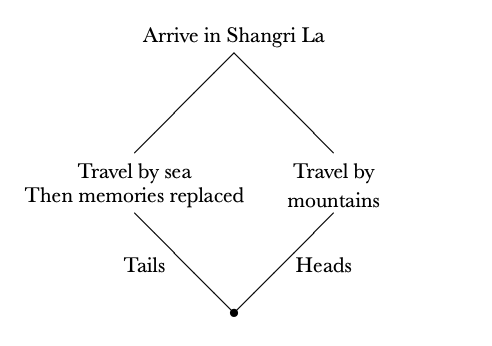
\includegraphics[keepaspectratio]{images/mbt-fig1.png}}

}

\caption{Original Shangri La game; Hugh takes the right-hand path}

\end{figure}%

There is something very puzzling about Hugh's case. On the one hand many
philosophers (including Arntzenius and Titelbaum) report a strong
intuition that once in Shangri La, Hugh should have equal confidence
that he came by the mountains as that he came by the sea. On the other
hand, it's hard to tell a dynamic story that makes sense of that. When
he is on the Path by the Mountains, Hugh clearly knows that he is on
that path. It isn't part of the story that the paths are so confusingly
marked that it is hard to tell which one one is on. Then Hugh gets to
Shangri La and, well, nothing happens. The most straightforward dynamic
story about Hugh's credences would suggest that, unless something
happens, he should simply retain his certainty that he was on the Path
by the Mountains.

And you might think evidentialism is committed to the same thing as that
dynamic story. To see why, imagine that Hugh is being terrifically
sneaky, and wearing a small camera in his glasses. The camera is
tracking what he sees, and Laurie is watching it on a distant TV
monitor. The guardians can't do anything to Laurie's memory, so they
don't, just like they don't do anything to Hugh. That night, it might
seem Hugh and Laurie have the same evidence. Yet, according to some
intuitions, it is rational for Laurie to believe that Hugh took the Path
by the Mountains, and not rational for Hugh to believe this.

Here's a natural way out of that bind. Say that the evidence Hugh and
Laurie have does not consist of what they saw as Hugh was ascending, but
their current mnemonic seemings. Now their evidence is different. Hugh
has the evidence that it seems to Hugh that Hugh ascended via the
mountains, and Laurie has the evidence that it seems to Laurie that Hugh
ascended via the mountains. And it is common knowledge that in either
this world or a nearby one, Hugh's mnemonic seemings are unreliable,
while Laurie's are reliable in all nearby worlds. So the temporally
local theories can handle the problem, while one might think temporally
extended theories cannot.

The most straightforward way to explain the common intuition about
Shangri La is via the indirect theory of memory. On that theory, Hugh
won't know that he came to Shangri La via the mountains. That's because
the report of his memory, ``We got here via the mountains, Hugh!'',
would be the same however he came up, and Hugh knows it. There is no
basic entitlement, on this theory, to move from \emph{My memory says
that p} to \emph{p}, and since Hugh does not even believe that a
correlation obtains in practice between what he believes about his
method of ascent and how he actually ascended, there is no earned
entitlement.

It is a little tempting to read some of the published arguments that
Hugh can't know he came via the mountains as reasoning in just this way.
Here is Arntzenius's central argument. (Assume Arntzenius is talking to
Hugh here, so `you' picks out Hugh.)

\begin{quote}
For you will know that he would have had the memories that you have
either way, and hence you know that the only relevant information that
you have is that the coin was fair.
(\citeproc{ref-Arntzenius2003}{Arntzenius 2003, 356})
\end{quote}

Sarah Moss (\citeproc{ref-Moss2012}{2012}) makes a similar claim about
the case. (Again, her narration is addressed to Hugh.)

\begin{quote}
Intuitively, even if you travel on the mountain path, you should have .5
credence when you gets to Shangri La that the coin landed heads. This is
a case of abnormal updating: once you arrive in Shangri La, you can no
longer be sure that you travelled on the mountain path, because you can
no longer trust your apparent memory. (\citeproc{ref-Moss2012}{Moss
2012, 241--42})
\end{quote}

Now it isn't immediately clear why the fact that Hugh would have the
same apparent memories in the two cases should matter. As far as I can
see, the only way it could matter is if the following two things were
true. First, we are using a temporally local theory, so the evidence is
what Hugh's memory reports when he is in Shangri La, not the evidence he
acquired on the trip up the mountain. And second, what those appearances
support is solely a function of things internal to the agent, and not,
say, their connection to the truth. As an evidentialist, I'm committed
to a version of that second assumption - at least, I'm committed to
saying that things that over-ride evidence must themselves be evidence.

Let's focus for now on the assumption of temporal localism behind the
arguments here. I'm going to offer a series of arguments against it,
starting with a variant on the Shangri La case.

\section{Iterated Shangri La}\label{iteratedshangrila}

Here's a slightly more complicated variant of the Shangri La example.

\begin{quote}
Sati walks up to the base of the paths to Shangri La. ``Have some toast
and yeast extract,'' says one of the attendants, somewhat stiltedly.

``Yeast extract?'' says Sati.

``Yes, yeast extract. Vegemite or Marmite, your choice.''.

``Must I?'' says Sati.

``You must.''

``Well, Vegemite then,'' says Sati, recalling fond memories of having
Vegemite in Australia, and dire memories of that trip to the English
countryside.

``Good choice,'' says the attendant. Sati has her Vegemite on toast, and
heads up the mountain path to Shangri La, as directed. On the way, she
notices a worried looking person standing in front of a priest about to
flip a coin. When she gets to Shangri La, she asks the attendant about
that.

``Oh,'' says the attendant, ``he chose Marmite.'' Sati looks confused as
to why this is relevant, so the attendant continues. ``The priests don't
like people who choose Marmite, but they still must let them through. So
they flip a coin to decide whether they will go by the sea or the
mountains. Then, if they went by the sea, they will wipe the memory of
that trip, and replace it with a memory of going through the
mountains.''

``I'm glad that didn't happen to me. Lucky I chose Vegemite.''

``Recently,'' continued the attendant, ``the priests decided to make
things more complicated. They decided they would also wipe the memory of
having eaten the Marmite, and hence facing the coin flip. Instead they
would implant a false memory of having chosen Vegemite, indeed false
memories of having preferred Vegemite to Marmite in the past, plus a
false memory of seeing some other poor sap facing the coin flip. They
really really don't like Marmite eaters.''

``So all the Marmite eaters get memories wiped?'' asked Sati.

``No, only if the coin lands the wrong way. So some people get to the
top thinking they liked Marmite. But we only tell that memories of going
by the sea will be wiped. In fact, knowing they chose Marmite is
evidence they went by the Mountains, but they don't know that.''

``It all sounds horrible,'' says Sati. ``I'm so glad I remembered I
liked Vegemite more than Marmite.''

``Have a good day!'' said the attendant, grinning.
\end{quote}

I think that Sati's last statement is correct; she does remember that
she likes Vegemite more than Marmite. Indeed, she knows this in virtue
of her memory. But it's not clear how a temporally local theory, either
direct or indirect, can get that answer.

Imagine someone, call him Joe, who starts off in the same situation as
Sati at the base of the mountain. Sadly, due to an unfortunate
unbringing, he prefers Marmite to Vegemite, so he takes that. And then
the coin lands the wrong way, and he is sent by the sea. Then his
memories are wiped and replaced with fake memories when he gets to
Shangri La.

\begin{figure}[H]

{\centering \pandocbounded{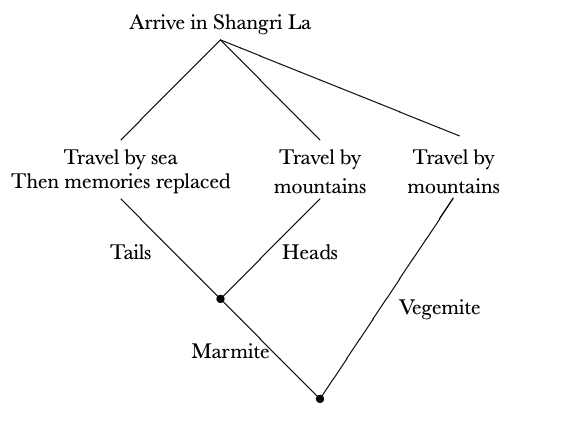
\includegraphics[keepaspectratio]{images/mbt-fig2.png}}

}

\caption{Revised Shangri La game; Sati takes the right-hand path, Joe
the left- hand path}

\end{figure}%

If a temporally local theory is correct, then presumably Sati and Joe
have the same evidence. And that means if evidentialism is true, then it
is rational for them to believe the same things. Yet that is
implausible; Joe should not be very confident that he had the Vegemite,
came by the mountains, and so on.

On the other hand, it is overdetermined that Sati can know she came by
the Mountains. The crucial difference between Sati and Hugh comes from
the defeasibility conditions on the transmission theory. Past memories
that \emph{p} transform into current evidence that \emph{p} unless they
are forgotten, or the agent gets some good reason to suspect that her
memory is unreliable. Hugh has such a reason; he is a coin flip away
from having faulty memories. Sati does not have such a reason. She knows
that had she had a very different kind of upbringing, and had she been
on the bad end of a coin flip, she would have had faulty memories. But a
reason to think that had things been different she would have reason to
distrust her memories is not, itself, a reason to distrust her memories.

Sati's case is not meant to be a close call. There are lots of relevant
ways in which her case is different to cases in which the defeasibility
clause is triggered. The fact that two different kinds of things need to
have gone wrong here is relevant. And the fact that the first requires
things going wrong for a long long time into the past is relevant. And
the fact that the first is only a problem in very different possible
worlds to actuality is relevant. In short, any plausible kind of
defeasibility condition whatsoever on the transmission theory will mean
that Joe's memories of going by the sea are not transmitted, but only an
implausibly strong defeasibility condition will prevent Sati's memories
from being transmitted.

Note that I have not said that Sati can trust her memories because the
probability of them being unreliable is so low. That is not the way to
formulate defeasibility conditions. The sense of probability that is
relevant here is evidential probability. And evidential probability is,
as the name suggests, explanatorily posterior to evidence possession. We
should not use evidential probability in our theory of what evidence the
agent has. Sati knows she grew up liking Vegemite, despite the Shangri
La shenanigans. But that's not because it is so improbable that she had
her memories wiped. Rather, it is improbable she had her memories wiped
because she knows she does not meet the conditions under which memories
are wiped.

So temporally extended theories can distinguish Sati's case from Joe's,
as intuition requires that they be distinguished. But temporally local
theories seem to have a problem here. Perhaps the problem here is not
with the theory of mnemonic evidence that the the temporally local
theories hold, but with evidentialism. Perhaps, that is, this is a case
where we should say that Sati and Joe have the same evidence, but that
this evidence supports different beliefs given the different reliability
of their memories.

But there is little to be said to motivate such a theory. If we aren't
going to be evidentialists, it isn't clear what the relevance of a
theory of evidence is. And if we are going to say that historical
events, like the fact that Joe's memories were wiped and Sati's weren't,
are relevant to contemporary rationality, it isn't clear what we gain by
having a temporally local theory of evidence. Either way, we have said
that the existence of past events is relevant to the rationality of
current beliefs. At this point we aren't engaged in much more than a
terminological dispute with the temporally extended theories.

\section{Against Indirect Theory}\label{againstindirecttheory}

As Matthias Steup (\citeproc{ref-Steup2013}{2013}) argues, the indirect
theory of memory is implausible. It says that when one remembers that,
say, the Chicago White Sox won the 2005 World Series, there are two
things that are needed in order to ground the rational belief. The first
is the apparent memory, and the second is some kind of reason to think
that the memories are reliable. But the only reasons we could have for
believing the second comes from what we have learned about the track
record of memory, or perhaps of the role of memory in human functioning.
And we couldn't be rational in believing those things unless we could
rationally rely on memory in forming beliefs. So we can never rationally
form any belief on the basis of memory unless we antecedently have
reason to trust memory. And that, plus the indirect theory of memory,
leads to a vicious regress, and hence to an implausible scepticism.

The argument here is similar in form to an argument that has often been
levelled against the indirect theory of testimony. This argument traces
back at least to Coady (\citeproc{ref-Coady1995}{1995}). The argument is
that children can rely on testimony to get knowledge, and hence rational
belief, but they don't have the information or the cognitive capacity to
rationally judge who is and isn't reliable. So it can't be, contra the
indirect theorist, that such judgments of reliability are required in
order to get rational belief and knowledge from testimony.

One problem with such an argument in the case of testimony is that it
has relied, historically, on a very impoverished view of the cognitive
capacities of young children. It is true that the capacity shown for
explicit reasoning by children is often very weak. But they have rather
amazing capacities for implicit reasoning, and there isn't any reason to
think they could not judge and track reliability of
informants.\footnote{On children's capacities to learn, see Saffran
  (\citeproc{ref-Saffran1996b}{1996}; \citeproc{ref-Saffran1996a}{1996})
  and Gopnik et al. (\citeproc{ref-Gopnik2001}{2001}). For applications
  of this directly to the judgments of credibility, see among many
  others, Koenig, Clément, and Harris
  (\citeproc{ref-KoenigClementHarris2004}{2004}) and Harris and
  Corriveau (\citeproc{ref-HarrisCorriveau2011}{2011}). Jaswal,
  McKercher, and VanderBorght (\citeproc{ref-Jaswal2008}{2008}) show
  that children don't just track credibility of informants, they trade
  off credibility of informant against credibility of what is currently
  being said. In general, the lesson from the last 10 to 20 years of
  research is that children have more than enough capacity to perform
  the cognitive tasks that indirect theorists require of them.}

The issue here is not capacity, it is information. No matter how much
capacity you have, you can't make rational judgments about the
reliability of memory without information about memory. And you can't
have that information without being able to use memory. That's the key
problem.

We can use this idea to strengthen the arguments in the previous section
about Sati. If the indirect theory of memory is wrong, we have to be a
bit careful about why Hugh can't know he came by the mountain path. It
can't just be that he lacks a reason to think his memories are reliable.
Rather, it must be that what he was told at the bottom of the mountain
is a reason to think his memories are not reliable. It must be the
presence of reasons to doubt memory, not the absence of reasons to
trust, that is doing the work.

And, as noted, this is a big difference between Hugh's case and Sati's.
Sati does not have any positive reason to doubt her memory. She is
several steps removed from the situation where her memories would be in
doubt. It's true that her mnemonic beliefs are insensitive to the truth
in a certain way. Arguably, the nearest world in which she came to
Shangri La by the sea is one where she still believes she came by the
mountains. But any kind of defeasible, direct theory of memory will
allow for some rational but insensitive belief.

Assume that our theory says that \emph{S} can rationally use her memory
to believe that \emph{p} unless defeaters \emph{D} are triggered. And
\emph{S} uses her memory to (accurately) remember ¬\emph{D}. That is,
she remembers that she is not in a situation where those defeaters are
triggered. Presumably if \emph{D} were true, her memory would be
unreliable; that's what makes \emph{D} a defeater. So there isn't any
reason to think that this mnemonic belief in ¬\emph{D} is sensitive; she
may well still have had it were \emph{D} true. But the direct theory
implies this doesn't matter, and the direct theory is the only theory on
the table given that the indirect theory leads to implausible
scepticism.

Could it be that Sati should not trust her memory because she is, and
she knows she is, in a class of people whose memories are unreliable?
Well, the mere fact that she is in such a class is not interesting. She
knows, after all she is a member of the class consisting of her and all
people with unreliable memories, and the memories of that class are as a
group unreliable. But that's not a reason to distrust her memory. Or, at
least, it can't be on pain of scepticism. What must matter is that she
is in such a class, and it is epistemologically significant. But the
significant class around here seems to be the class of people whose
memories have been erased, or who have reason to suspect their memories
have been erased. And that doesn't include Sati. She knows she likes
Vegemite, and has for a long time, and she knows that only
Marmite-likers in Shangri La had their memories erased.

Here's what is true of Sati. She is, right now, phenomenally
indistinguishable from a possible person whose memories are unreliable.
But why should that matter? We all know brain in vat cases are possible,
and each of us is phenomenally indistinguishable from such an unreliable
`person'. But that isn't on its own grounds for doubt about memory. All
that she learns from the attendant is that another kind of brain in vat
case is possible. But she knew they were possible all along. The case
isn't actual and, unless we come up with a trigger for the defeater in
the theory of memory, she has no reason to think it is actual.

\section{Argument from A Priority}\label{argumentfromapriority}

There is another argument against the temporally local theories, and
against both the direct and indirect theories, that we can derive from
the work of Tyler Burge (\citeproc{ref-Burge1993}{1993},
\citeproc{ref-Burge1997}{1997}). (I should note that there is
considerable dispute about how best to interpret Burge. I'm not claiming
that what follows is the best interpretation, or the only
interpretation, just that it is an interesting argument inspired by, and
quite arguably contained in, his work.)

Tamati is doing a proof. At one stage in the proof he appeals to
Fermat's Little Theorem, which says for any natural number \emph{n}, and
any prime \emph{p}, \emph{n\textsuperscript{p}}~≡~\emph{n}~mod~\emph{p}.
Using this theorem, Tamati completes his proof, and derives a nice
result \emph{M}. Intuitively, Tamati has not just come to know \emph{M},
but he has come to know \emph{M} a priori.

But assume, now, that either kind of temporally local theory is true. At
one stage of the proof, Tamati had to, at least implicitly, reason as
follows. It seems to me that I remember that
\emph{n\textsuperscript{p}}~≡~\emph{n}~mod~\emph{p}, so (perhaps with an
extra premise), \emph{n\textsuperscript{p}}~≡~\emph{n}~mod~\emph{p}. And
that can't be a priori reasoning, since the premise about how things
seem to Tamati is contingent and a posteriori. If the indirect theory of
memory is right, the extra premise needed about the reliability of
Tamati's memory will also be contingent and a posteriori.

It would be a very strange and revisionary theory of the a priori to say
that any proof is not a priori if it relies on remembered theorems
without, perhaps, memory of the proof of that theorem. The proof of
Fermat's Little Theorem isn't difficult, but it does go through several
steps. It is hard to keep the whole proof in mind at once. Even proving
it, that is, requires a little memory. On the temporally local theory,
it isn't clear that it could ever be a priori knowable for any normal
person. And any theorem that required using it would similarly be a
posteriori.

Perhaps it could be said that Tamati's reasoning is a priori because it
doesn't rely on sense perception, only on perception of how things seem
to Tamati. But some such perception of how things seem yields a
posteriori knowledge. If Tamati has a headache, and notices this at the
same time he remembers Fermat's Little Theorem, he gets a posteriori
knowledge of the contingent truth that he has a headache, and a priori
knowledge of the necessary truth of the theorem.

In short, a transmissive theory of memory is required to get the result
that Tamati gets a priori knowledge of the mathematical theorem. As
Burge argues, a transmissive theory of testimony gets the exciting
result that when Tamati goes on to tell his friend about \emph{M}, the
friend gets a priori knowledge of \emph{M} as well. If one thinks it is
intuitive that the friend's knowledge is a priori, that's a good reason
to favour a transmissive view of testimony. But that the friend's
knowledge is a priori is not as intuitively obvious as that Tamati's
knowledge is a priori, so it isn't obvious we must treat memory and
testimony the same way here.

I'll end this section with a note about the dialectic. What would the
argument of the paper lose if the arguments of this section didn't work?
This is an important question because of arguments, such as those by
Daniele Sgaravatti (\citeproc{ref-Sgaravatti2012}{2012}, Ch. 3), that
the a priori/a posteriori distinction can't do the epistemological work
that it is traditionally taken to do. The answer is that we'd lose one
of the best arguments against the direct version of the temporally local
theory, while the argument against the indirect version would not be
significantly affected.

Assume for now that one is happy with Tamati's knowledge, and indeed all
non-trivial mathematical knowledge, being a posteriori in this way,
because it relies on mnemonic knowledge about one's earlier self. There
is still the question of how one gets from this knowledge about one's
earlier self to knowledge of mathematics. On this indirect theory, this
goes via reasoning about the reliability of one's earlier self. But that
reasoning will have to use some non-trivial mathematics, and we'll be
back in the kind of circle we warned about in the previous section. On
the direct theory, this won't be a problem, since there isn't any
challenge in getting from \emph{I have an apparent memory that p} to
\emph{p}. That inference is perfectly sound, as long as one lacks
reasons to distrust it. It is still, I think, puzzling that we have to
analyse mathematicians as reasoning this way, and generating a
posteriori knowledge. But they key dialectical point is that sense of
puzzlement is only relevant to thinking about the direct version of the
temporally local theory; the indirect version is beset by a host of
further and more serious problems.

\section{Argument from Laundering}\label{argumentfromlaundering}

The arguments involving Sati and Tamati were designed to show that not
all rational mnemonic belief relies on inference from the existence of a
current mnemonic seeming. But neither argument suggested that there was
anything wrong with such inferences. It is fully compatible with what I
said about both Sati and Tamati that they could also try to infer from
how things seem to them to facts about how they got to Shangri La, or
about modular arithmetic.

Barnett's argument for a temporally extended view takes the opposite
tack. He thinks there is something problematic about these inferences,
or at least a special class of them. And because of this, he infers that
the inference from present seeming can't be explanatorily important. And
that gets him to a version of a temporally extended theory.

So what's the problem? Here's the schematic case that he focusses on.

\begin{quote}
\begin{description}
\tightlist
\item[Two Beliefs]
On Monday you came to believe that \emph{p} for good reasons that
justified your belief, and on Tuesday you came to believe that \emph{q}
for bad reasons that failed to justify it (where \emph{p} and \emph{q}
are independent). It is now Wednesday, and you have forgotten nothing,
reconsidered nothing, and learned no new relevant evidence. You recall
each conclusion without occurrently recalling your original reasons for
those conclusions. (\citeproc{ref-Barnett2015}{Barnett 2015, 15})
\end{description}
\end{quote}

Again, it's a bit of an annoyance to use `you', especially since you,
dear reader, would not do anything so foolhardy as come to believe
\emph{q}. So let's assume Barnett's narration is directed at Kim. And
the question is, is Kim's belief that \emph{q}, on Wednesday, rational?
Assume, to make the case most interesting, that this mistaken inference
to \emph{q} is completely out of character. Kim is, and knows he is, a
very reliable processor of information, who rarely makes this kind of
mistake.

The worry is that any temporally local theory will say that Kim's belief
on Wednesday is rational. After all, Kim has an apparent belief that
\emph{q}, and not only lacks evidence of his unreliability, but knows he
is reliable. Great! But, intuitively, his belief doesn't go from being
irrational to being rational just by the passage of time. It can't get
its irrationality laundered out in this way.

But it isn't clear how big a problem this really should be. Note that
Kim is supposed to have forgotten nothing. So the evidence on which
\emph{q} was based is still there. Now allow the temporally local theory
a principle that they should want on independent grounds. That principle
is that evidence screens judgment; the evidential force of the fact that
an agent made a judgment is completely screened, for that agent, by the
evidence the judgment was based on.\footnote{I haven't actually defended
  this in print yet, but it is correctly attributed to me by Sophie
  Horowitz (\citeproc{ref-Horowitz2013}{2014, 25}).} I just stated that
principle synchronically, so it doesn't immediately have implications
for Kim's case. But it is plausible to say that as long as the judgment
remains, its evidential force is screened off by the evidence it was
based on.

Now whether one has a direct or indirect theory, Kim is not obviously
compelled to hold on to her belief that \emph{q}. And whether or not one
believes the screening principle, the fact that Kim has forgotten
nothing means that there is no symmetry between the cases of \emph{p}
and \emph{q}. The relevant evidence is different in the two cases. The
only theorist who has a challenge here is one who thinks that only
occurrent states are evidence, and that is a particularly implausible
addition to the indirect theory.

Barnett's case is different in a couple of respects than an example
Gilbert Harman (\citeproc{ref-Harman1986}{1986}, Ch. 4) uses to draw
rather different conclusions. Working through the differences between
them allows us to see something interesting about rational dilemmas,
even if it isn't immediately relevant to the debates about memory.

In Harman's example, Karen first draws a conclusion \emph{q}. This is
actually rational for her to draw given her evidence, but her evidence
was extremely misleading. She then forgets why she came to believe
\emph{q}, and gets new evidence that would show her the old evidence was
misleading. But since she doesn't remember why she believed \emph{q},
she doesn't know that this new evidence affects her grounds for belief
in \emph{q}, and retains the belief.

Harman says that this is rational. Karen isn't required to keep track of
her evidence for each thing she believes. That seems right. It is hardly
a rational failing of mine to not remember precisely why I think that
the White Sox won the 2005 World Series; I don't need to keep that level
of detail in mind. And if Karen does not do that, she can't be expected
to adjust her beliefs when the evidence that, unbeknownst to her, they
are based on is undermined.

Harman thinks that our original intuition about Karen's case is that her
belief in \emph{q} is irrational once it has been undermined. But he
also thinks reflection on real life cases like Karen's shows this
intuition to be mistaken. The lesson he draws from this is that
something like the direct theory is right; Karen can trust her memories
unless she has a special reason to doubt them, even if in fact she
couldn't put together a positive argument for their reliability.

Barnett's case of Kim is different than Harman's case of Karen in two
respects. Kim retains his evidence; Karen loses hers. And Kim makes an
irrational mistake; Karen is rationally misled by misleading evidence.
Are those differences enough to think we should treat the cases
differently? Or should we be worried that Karen's case, like perhaps
Kim's, is one where intuition is not a reliable guide?

I don't actually have a firm view on this. The differences are
significant. Harman himself thinks that the intuition in Karen's case is
driven by the mistaken assumption that Karen will track and retain her
evidence. That's not true in normal cases like Karen's. But it is true,
by stipulation, in Kim's. So that is one big reason for treating the
cases differently. Still, I do worry a little that we're drifting into
areas where intuition is unreliable.

To make that worry a little more concrete, consider this argument for
the conclusion that Kim's belief in \emph{q} is actually rational.

\begin{enumerate}
\def\labelenumi{\arabic{enumi}.}
\tightlist
\item
  It would be irrational for Kim to re-open inquiry into whether
  \emph{q}, given that it was settled, and no new evidence has come in.
\item
  It would be irrational or impossible for Kim to intentionally forget
  \emph{q}.
\item
  Kim cannot change his attitude to \emph{q} without either re-opening
  inquiry into whether \emph{q}, or by forgetting \emph{q}.
\item
  There is some rational attitude towards \emph{q} that Kim can take.
\item
  So, Kim is rational to retain belief in \emph{q}, since any other
  possible path would involve irrationality of some kind.
\end{enumerate}

Premises 2 and 3 aren't, I think, particularly controversial, especially
if `inquiry' is read so broadly that any re-evaluation of \emph{q}
counts as re-opening inquiry. The issues are premises 1 and 4. Premise 4
is a no dilemmas principle. We'll return to it later, though in this
context it is notable that Barnett himself endorses it, as do many other
epistemologists. (\citeproc{ref-Barnett2015}{Barnett 2015, 10})

The big issue is premise 1. I think it is true. It is a mistake to go
around constantly reconsidering things that one has settled. Once a
decision has been reached, it should be held, unless a reason comes
along to reconsider it. That reason may be evidence that the decision
was faulty, or reason to think the decision was badly made. But the mere
passage of time is not a reason to reconsider, and nor is the fact that
if inquiry were (properly) conducted, it would yield a different
conclusion.

The picture I'm putting forward here owes a lot to Richard Holton
(\citeproc{ref-Holton1999}{1999}, \citeproc{ref-Holton2009}{2009},
\citeproc{ref-Holton2014}{2014}), as well as to a related idea due to
Crispin Wright (\citeproc{ref-Wright2004}{2004}). Holton argues that if
one has an intention, rationality requires one to maintain that unless a
good reason comes along to reconsider it. The fact that one would not
form the intention again were one to reconsider it is not, he thinks,
itself a good reason. Strikingly, he says that even in Kavka's toxin
puzzle (\citeproc{ref-Kavka1983}{Kavka 1983}), the agent who intends to
drink the toxin should not reconsider, because they have no reason to do
so. (\citeproc{ref-Holton2009}{Holton 2009, 162--65}). And he suggests
that we should think of belief along similar lines
(\citeproc{ref-Holton2014}{Holton 2014}). To believe something is to
commit to its truth, and we need a positive reason to give up our
commitments. Wright argues that the sceptic tries to lure us into
opening inquiries we can tell will not be completed. We should resist
the lure. We have no reason to open the broad ranging inquiry into our
own competencies that the sceptic wants us to hold, and good reason to
avoid it.\footnote{Sue Hamilton (\citeproc{ref-Hamilton2001}{2001, 78})
  says that this idea, that it is wrong to open an inquiry you know you
  can't complete, plays a central role in the epistemology of the
  important Nyāya philosopher Gotama. The discussion of forecasting in
  Tetlock and Gardner (\citeproc{ref-Tetlock2015}{2015}) might cast
  doubt on whether the kind of conservatism I'm endorsing here is
  empirically sound. There is a suggestion there that people who tinker
  with their credal states more frequently end up with more accurate
  credences. This is a topic that deserves revisiting as more data comes
  in.}

We can perhaps motivate the application of these ideas to cases like
Kim's by thinking of a similar case involving action.

\begin{quote}
Ned has been thinking about buying a new bed. He is deciding between a
wood bed and a metal bed. And he just decided to get the wood bed. This
is a bad mistake. He will like the metal bed much better, and this is in
fact clear from the evidence available to Ned. But he's made up his
mind. The wood bed store is five miles east, the metal bed store is five
miles west. And there's Ned in his car, driving eastward. What does
rationality require of Ned now?
\end{quote}

I think Ned's in a rational dilemma. It is irrational to drive to the
wood bed store and buy a wood bed. He won't like it, and it is
predictable that he won't. What a mistake. But it is irrational to
reopen inquiry. He's made up his mind, and now he should focus on the
road. He hasn't received any new evidence about the qualities of the
bed, or any reason to think he mis-evaluated the old evidence. And we
can't go around second guessing our past decisions all the time. That
includes those of us (presumably all of us) who make mistakes. It is
irrational to be fickle.

So what can Ned rationally do? The arguments of the previous paragraph
suggest he's in a rational dilemma. If you want to act rationally, you
shouldn't start where Ned is. If he keeps driving to the wood bed store,
he'll irrationally buy a sub-optimal bed. If he thinks again about the
issue, he'll be irrationally fickle. Rationality requires something that
is practically impossible; changing his mind about what to buy without
re-opening the issue of what to buy.

This is a dilemma for Ned, but it is one he could have avoided. He could
have not made the mistaken decision in the first place. It may or may
not be unfair if rationality makes incompatible demands on an agent
without any chance to avoid them. But it isn't unfair to think that
agents who make mistakes at \emph{t}\textsubscript{1} are, in virtue of
those mistakes, left without any good options at
\emph{t}\textsubscript{2}. Mistakes have consequences.

Is this inconsistent with evidentialism? I said above that evidentialism
says the rational status of a belief supervenes on the evidence that the
agent has. Yet now I'm saying Ned is irrational to change his mind. But
if he had, with the very same evidence, believed that he should get the
metal bed, that would have been rational. This looks like a
counterexample to evidentialism.

Here's why it isn't a counterexample. What is irrational for Ned is
re-opening inquiry into what bed to get. It is the activity of engaging
in further consideration of the question that it is irrational.
Moreover, this is irrational because the evidence that is available to
make this decision does not support it. Should Ned irrationally engage
in this activity, there is a uniquely rational way to finish it, which
is to change his mind. But that's not the same as saying that he should,
rationally, change his mind.

I am making a big assumption here, but one I think is true. Careful
consideration involves thinking through a large amount of evidence.
Decisions to engage in careful consideration must be made on the basis
of flimsier amounts of evidence. After all, to bring all the evidence
one has to bear on a question is to engage in careful consideration. So
a decision to engage in such consideration must not use all that
evidence. So evidentialism must say that the rationality of a belief,
credence, decision etc must depend on, i.e., supervene on, the evidence
available to the agent when they make that decision. And when deciding
whether to carefully consider or reflect on the evidence, very little is
available.

That's why I think Ned isn't a counterexample to evidentialism. And nor
is Kim a counterexample to evidentialism, even if there is no way she
can rationally lose her belief in \emph{q}. For Kim too faces a dilemma,
of just the same kind. So the argument I gave for the rationality of
Kim's continuing to believe \emph{q} goes wrong at step 4. Kim has
gotten herself into a mess, and there are no rational ways out.

But note that last conclusion cuts across the theories of memory we've
considered here. The temporally extended theory has, as its distinctive
claim, that some agents have a kind of evidence that the temporally
local theory says no agent has. But Kim is not one of those agents. The
evidence in question is evidence one gets when one acquires a piece of
knowledge, and keeps that token mental state across time. And the
relevant fact about Kim is that he has a belief in \emph{q} that is well
and truly not a piece of knowledge. So it doesn't look like the case
should tell the local and extended theories apart.

What it does so is show that there is a new kind of argument for the
possibility of rational dilemmas. People make mistakes. When they do,
there might be no good way to undo the effect of the mistake. And then
they're in a dilemma. We don't avoid that conclusion by giving people
who don't make mistakes more evidence.

\section{Conclusion and Future
Research}\label{conclusionandfutureresearch}

I've argued for a transmissive, temporally extended, view of memory and
the evidence it provides. When I remember that the White Sox won in
2005, it is the fact that they won which is my evidence, not my apparent
memory. The role of memory is to preserve this fact in evidence, not to
give me new evidence for it. Saying this invites any number of
questions. I'll end with a list of several ones that I find fascinating,
but which I'm a long way from having answers to, divided up loosely into
questions about metaphysics, and questions about epistemology.

\subsection{Preservation}\label{preservation}

What is it for memory to preserve a belief? Sven Bernecker
(\citeproc{ref-Bernecker2008}{2008}) has written on this at length, and
the issue turns out to be much more complicated than we might first
suspect. I'm particularly unsure about cases like this one,

\begin{quote}
\begin{description}
\tightlist
\item[Ankati.]
I haven't had to change planes at O'Hare for over five years. That makes
me happy.
\item[Bojan.]
Are you sure? What about the trip to Vancouver? Or the one to Hong Kong?
\item[Ankati.]
Vancouver was a direct flight. And I went to Hong Kong via New York.
But, oh, you're right, I came back via O'Hare. Sad face.
\end{description}
\end{quote}

At the end Ankati remembers that she flew home from Hong Kong via
O'Hare. Is this a belief that was stored in memory ever since it
happened? If so, we have to say that Ankati had inconsistent beliefs at
the start of the conversation. If not, then I think it is hard to say
that the relevant evidence for the belief that saddens her is the fact
that she transferred at O'Hare. In such a case, it seems to me that the
temporally local theory is more plausible than in more usual cases.

\subsection{Initial Evidence and
Over-Riding}\label{initialevidenceandover-riding}

The following two questions are related:

\begin{itemize}
\tightlist
\item
  What past states can constitute present evidence?
\item
  What present states can over-ride, or defeat, past evidence?
\end{itemize}

My instinct is to defend an extremely restricted answer to this pair of
questions. In particular, \emph{S}'s attitude towards \emph{p} at
\emph{t}\textsubscript{1} can only be evidence for her at
\emph{t}\textsubscript{2} if the following conditions obtain.

\begin{enumerate}
\def\labelenumi{\arabic{enumi}.}
\tightlist
\item
  \emph{S} knows that \emph{p} at \emph{t}\textsubscript{1}.
\item
  \emph{S} does not receive a significant amount of evidence against
  \emph{p} between \emph{t}\textsubscript{1} and
  \emph{t}\textsubscript{2}.
\item
  \emph{S} does not receive (undefeated) reasons to distrust her ability
  to preserve information between \emph{t}\textsubscript{1} and
  \emph{t}\textsubscript{2}.
\end{enumerate}

But every one of these points is problematic.

The first point might imply some counterintuitive things about people
who trust misleading evidence, such as `Karen' in the earlier cited
example by Gilbert Harman (\citeproc{ref-Harman1986}{1986}, Ch. 4).
Let's focus on an even simpler case than Harman's. Unlike me, my
doppleganger Nairb believes that the Astros beat the White Sox in the
2005 World Series. That's because his web browser had been hacked on
that crucial October morning, and it reported the wrong results. He
hasn't seen any relevant evidence since. He has forgotten why he thinks
the Astros won in 2005, but has held on to the belief. Is this belief
rational, and what's his evidence for it?

The evidence can't be that the Astros won in 2005; they didn't. And it
can't be that his computer reported that; he's forgotten that fact.
Let's say that it is his apparent memory that they won, which seems to
be the only remaining option. That would mean that the rationality of
his forming the belief in the first place is independent of whether his
current belief that the Astros won is rational. That's better than the
alternative options, but it isn't particularly happy either.

The second point leads us into the version of the dogmatism puzzle that
Maria Lasonen-Aarnio (\citeproc{ref-Lasonen-Aarnio2014a}{2014b}) has
developed. Assume that significant evidence can factor into
insignificant parts. Pazu knows that \emph{p}, then gets three pieces of
evidence \emph{e}\textsubscript{1}, \emph{e}\textsubscript{2} and
\emph{e}\textsubscript{3} that tell against \emph{p}. The conjunction is
significant evidence, the individual parts are not. But the parts come
in sequentially. When \emph{e}\textsubscript{1} comes in, Pazu still
knows \emph{p}; after all, it is insignificant evidence. So Pazu can
conclude, i.e., know, that it is misleading evidence. And, intuitively,
we can ignore evidence we know to be misleading. So he ignores
\emph{e}\textsubscript{1}. And for similar reasons he ignores
\emph{e}\textsubscript{2}. Then \emph{e}\textsubscript{3} comes in.
Should he still ignore it? Presumably; it is on its own insignificant,
and the only other evidence was known to be misleading, and so ignored.
But it is odd that Pazu can hold onto his knowledge in \emph{p} in the
face of these three pieces of evidence, while he would have lost
knowledge had they come in at once.

Finally, we need to explain why evidence of unreliability of mnemonic
processes can block mnemonic knowledge. If memory was a source of
evidence, rather than a preserver of evidence, that would be an easy
problem. In general, a source does not provide evidence to an agent if
the agent has reason to believe that it is unreliable. The problem is
how to motivate an extension of that principle to memory, which is in
general not a source of evidence, but a preserver of it.

We could simply insist that the Shangri La case shows that the
preservative role of memory can be defeated given sufficient grounds to
doubt its accuracy. I think that's right, we can insist that. But there
is a puzzle still about why this should be so. And that puzzle remains
work for another day, as do the other puzzles in this section.

\subsection{Externalism}\label{externalism}

Finally, there are some tantalising possibilities for new angles into
familiar epistemological debates between internalists and externalists.
It is hardly news that this is possible; Goldman's `problem of forgotten
evidence' is a familiar challenge to (certain) internalists
(\citeproc{ref-Goldman1999}{Goldman 1999}). But there might be other
ways to make memory relevant to familiar debates.

If the temporally extended theory is true, then what is rational depends
on something that is, well, extended. And if what is rational depends on
something that is extended in time, we might think it is less surprising
that is also depends on something that is extended in space. And that
suggests the way to a kind of externalism.

We can do a bit better than that hand-waving metaphor though. There are
versions of the New Evil Demon problem for transmissivism. If
transmissivism is true anyway, that means those problems have solutions.
Then we just have to find what those solutions are, and see if they
generalise to solutions to the spatial version of the New Evil Demon
problem. And if they do, we might have new ways to defend externalist
theories of rationality, or at least new motivations for familiar ways
to defend those theories.

\subsection*{References}\label{references}
\addcontentsline{toc}{subsection}{References}

\phantomsection\label{refs}
\begin{CSLReferences}{1}{0}
\bibitem[\citeproctext]{ref-Arntzenius2003}
Arntzenius, Frank. 2003. {``Some Problems for Conditionalization and
Reflection.''} \emph{Journal of Philosophy} 100 (7): 356--70. doi:
\href{https://doi.org/10.5840/jphil2003100729}{10.5840/jphil2003100729}.

\bibitem[\citeproctext]{ref-Barnett2015}
Barnett, David James. 2015. {``Is Memory Merely Testimony from One's
Former Self?''} \emph{Philosophical Review} 124 (3): 353--92. doi:
\href{https://doi.org/10.1215/00318108-2895337}{10.1215/00318108-2895337}.

\bibitem[\citeproctext]{ref-Bernecker2008}
Bernecker, Sven. 2008. \emph{The Metaphysics of Memory}. New York:
Springer.

\bibitem[\citeproctext]{ref-Burge1993}
Burge, Tyler. 1993. {``Content Preservation.''} \emph{Philosophical
Review} 102 (4): 457--88. doi:
\href{https://doi.org/10.2307/2185680}{10.2307/2185680}.

\bibitem[\citeproctext]{ref-Burge1997}
---------. 1997. {``Interlocution, Perception, and Memory.''}
\emph{Philosophical Studies} 86 (1): 21--47. doi:
\href{https://doi.org/10.1023/A:1004261628340}{10.1023/A:1004261628340}.

\bibitem[\citeproctext]{ref-Coady1995}
Coady, C. A. J. 1995. \emph{Testimony: A Philosophical Study}. Oxford:
Clarendon Press.

\bibitem[\citeproctext]{ref-Dokic2001}
Dokic, Jérôme. 2001. {``Is Memory Purely Preservative?''} In \emph{Time
and Memory. Issues in Philosophy and Psychology}, edited by Christoph
Hoerl and Teresa McCormack, 213--32. Oxford: Oxford University Press.

\bibitem[\citeproctext]{ref-Dummett1994}
Dummett, Michael. 1994. {``Testimony and Memory.''} In \emph{{K}nowing
from {W}ords}, edited by A. Chakrabarti and B. K. Matilal, 1--23.
Dordrecht: {K}luwer.

\bibitem[\citeproctext]{ref-Fricker1994}
Fricker, Elizabeth. 1994. {``{A}gainst {G}ullibility.''} In
\emph{{K}nowing from {W}ords}, edited by A. Chakrabarti and B. K.
Matilal, 125--61. Dordrecht: {K}luwer.

\bibitem[\citeproctext]{ref-Goldman1999}
Goldman, Alvin. 1999. {``Internalism Exposed.''} \emph{Journal of
Philosophy} 96 (6): 271--93. doi:
\href{https://doi.org/10.2307/2564679}{10.2307/2564679}.

\bibitem[\citeproctext]{ref-Gopnik2001}
Gopnik, Alison, David M. Sobel, Laura E. Schulz, and Clark Glymour.
2001. {``Causal Learning Mechanisms in Very Young Children: Two-,
Three-, and Four-Year-Olds Infer Causal Relations from Patterns of
Variation and Covariation.''} \emph{Developmental Psychology} 37 (5):
620--29. doi:
\href{https://doi.org/10.1037//0012-1649.37.5.620}{10.1037//0012-1649.37.5.620}.

\bibitem[\citeproctext]{ref-Hamilton2001}
Hamilton, Sue. 2001. \emph{Indian Philosophy: A Very Short
Introduction}. Oxford: {O}xford {U}niversity {P}ress.

\bibitem[\citeproctext]{ref-Harman1986}
Harman, Gilbert. 1986. \emph{Change in View}. Cambridge, MA: Bradford.

\bibitem[\citeproctext]{ref-HarrisCorriveau2011}
Harris, Paul L., and Kathleen H. Corriveau. 2011. {``Young Children's
Selective Trust in Informants.''} \emph{Philosophical Transactions of
the Royal Society B} 366: 1179--87. doi:
\href{https://doi.org/10.1098/rstb.2010.0321}{10.1098/rstb.2010.0321}.

\bibitem[\citeproctext]{ref-Holton1999}
Holton, Richard. 1999. {``Intention and Weakness of Will.''} \emph{The
Journal of Philosophy} 96 (5): 241--62. doi:
\href{https://doi.org/10.2307/2564667}{10.2307/2564667}.

\bibitem[\citeproctext]{ref-Holton2009}
---------. 2009. \emph{Willing, Wanting, Waiting}. Oxford: Oxford
University Press.

\bibitem[\citeproctext]{ref-Holton2014}
---------. 2014. {``Intention as a Model for Belief.''} In
\emph{Rational and Social Agency: Essays on the Philosophy of Michael
Bratman}, edited by Manuel Vargas and Gideon Yaffe, 12--37. Oxford:
Oxford University Press.

\bibitem[\citeproctext]{ref-Horowitz2013}
Horowitz, Sophie. 2014. {``Epistemic Akrasia.''} \emph{No{û}s} 48 (4):
718--44. doi:
\href{https://doi.org/10.1111/nous.12026}{10.1111/nous.12026}.

\bibitem[\citeproctext]{ref-Jaswal2008}
Jaswal, Vikram K., David A. McKercher, and Mieke VanderBorght. 2008.
{``Limitations on Reliability: Regularity Rules in the English Plural
and Past Tense.''} \emph{Child Development} 79 (3): 750--60. doi:
\href{https://doi.org/10.1111/j.1467-8624.2008.01155.x}{10.1111/j.1467-8624.2008.01155.x}.

\bibitem[\citeproctext]{ref-Kavka1983}
Kavka, Gregory S. 1983. {``The Toxin Puzzle.''} \emph{Analysis} 43 (1):
33--36. doi:
\href{https://doi.org/10.1093/analys/43.1.33}{10.1093/analys/43.1.33}.

\bibitem[\citeproctext]{ref-KoenigClementHarris2004}
Koenig, Mellisa A., Fabrice Clément, and Paul L. Harris. 2004. {``Trust
in Testimony: Children's Use of True and False Statements.''}
\emph{Psychological Science} 15 (10): 694--98. doi:
\href{https://doi.org/10.1111/j.0956-7976.2004.00742.x}{10.1111/j.0956-7976.2004.00742.x}.

\bibitem[\citeproctext]{ref-Lackey2005}
Lackey, Jennifer. 2005. {``Memory as a Generative Epistemic Source.''}
\emph{Philosophy and Phenomenological Research} 70 (3): 636--58. doi:
\href{https://doi.org/10.1111/j.1933-1592.2005.tb00418.x}{10.1111/j.1933-1592.2005.tb00418.x}.

\bibitem[\citeproctext]{ref-Lackey2008}
---------. 2008. \emph{Learning from Words: Testimony as a Source of
Knowledge}. Oxford: Oxford University Press.

\bibitem[\citeproctext]{ref-Lasonen-Aarnio2010}
Lasonen-Aarnio, Maria. 2010. {``Is There a Viable Account of
Well-Founded Belief.''} \emph{Erkenntnis} 72 (2): 205--31. doi:
\href{https://doi.org/10.1007/s10670-009-9200-z}{10.1007/s10670-009-9200-z}.

\bibitem[\citeproctext]{ref-Lasonen-Aarnio2014}
---------. 2014a. {``Higher-Order Evidence and the Limits of Defeat.''}
\emph{Philosophy and Phenomenological Research} 88 (2): 314--45. doi:
\href{https://doi.org/10.1111/phpr.12090}{10.1111/phpr.12090}.

\bibitem[\citeproctext]{ref-Lasonen-Aarnio2014a}
---------. 2014b. {``The Dogmatism Puzzle.''} \emph{Australasian Journal
of Philosophy} 92 (3): 417--32. doi:
\href{https://doi.org/10.1080/00048402.2013.834949}{10.1080/00048402.2013.834949}.

\bibitem[\citeproctext]{ref-Lewis1996b}
Lewis, David. 1996. {``Elusive Knowledge.''} \emph{Australasian Journal
of Philosophy} 74 (4): 549--67. doi:
\href{https://doi.org/10.1080/00048409612347521}{10.1080/00048409612347521}.
Reprinted in his \emph{Papers in Metaphysics and Epistemology},
Cambridge: Cambridge University Press, 1999, 418-446. References to
reprint.

\bibitem[\citeproctext]{ref-Malmgren2006}
Malmgren, Anna-Sara. 2006. {``Is There a Priori Knowledge by
Testimony?''} \emph{Philosophical Review} 115 (2): 199--241. doi:
\href{https://doi.org/10.1215/00318108-115-2-199}{10.1215/00318108-115-2-199}.

\bibitem[\citeproctext]{ref-Moss2012}
Moss, Sarah. 2012. {``Updating as Communication.''} \emph{Philosophy and
Phenomenological Research} 85 (2): 225--48. doi:
\href{https://doi.org/10.1111/j.1933-1592.2011.00572.x}{10.1111/j.1933-1592.2011.00572.x}.

\bibitem[\citeproctext]{ref-Pryor2004}
Pryor, James. 2004. {``What's Wrong with Moore's Argument?''}
\emph{Philosophical Issues} 14 (1): 349--78. doi:
\href{https://doi.org/10.1111/j.1533-6077.2004.00034.x}{10.1111/j.1533-6077.2004.00034.x}.

\bibitem[\citeproctext]{ref-Saffran1996b}
Saffran, Jenny R., Richard N. Aslin, and Elissa L. Newport. 1996.
{``Statistical Learning by 8-Month-Old Infants.''} \emph{Science} 274
(5294): 1926--28. doi:
\href{https://doi.org/10.1126/science.274.5294.1926}{10.1126/science.274.5294.1926}.

\bibitem[\citeproctext]{ref-Saffran1996a}
Saffran, Jenny R., Elissa L. Newport, and Richard N. Aslin. 1996.
{``Word Segmentation: The Role of Distributional Cues.''} \emph{Journal
of Memory and Language} 35 (4): 606--21. doi:
\href{https://doi.org/10.1006/jmla.1996.0032}{10.1006/jmla.1996.0032}.

\bibitem[\citeproctext]{ref-Schmitt2006}
Schmitt, Frederick F. 2006. {``{T}estimonial {J}ustification and
{T}ransindividual {R}easons.''} In \emph{{T}he {E}pistemology of
{T}estimony}, edited by Jennifer Lackey and Ernest Sosa, 193--224.
{O}xford {U}niversity {P}ress.

\bibitem[\citeproctext]{ref-Sgaravatti2012}
Sgaravatti, Daniele. 2012. {``Down to Earth Philosophy: An
Anti-Exceptionalist Essay on Thought Experiments and Philosophical
Methodology.''} PhD thesis, University of St Andrews.

\bibitem[\citeproctext]{ref-Steup2013}
Steup, Matthias. 2013. {``Is Epistemic Circularity Bad?''} \emph{Res
Philosophica} 90 (2): 215--35. doi:
\url{http://dx.doi.org/10.11612/resphil.2013.90.2.8}.

\bibitem[\citeproctext]{ref-Tetlock2015}
Tetlock, Philip E., and Dan Gardner. 2015. \emph{Superforecasting: The
Art and Science of Prediction}. New York: Crown.

\bibitem[\citeproctext]{ref-Titelbaum2014}
Titelbaum, Michael. 2014. \emph{Quitting Certainties: A Bayesian
Framework for Modeling Degrees of Belief}. Oxford: Oxford.

\bibitem[\citeproctext]{ref-Weatherson2012}
Weatherson, Brian. 2012. {``Knowledge, Bets and Interests.''} In
\emph{Knowledge Ascriptions}, edited by Jessica Brown and Mikkel Gerken,
75--103. Oxford: Oxford University Press.

\bibitem[\citeproctext]{ref-White2005}
White, Roger. 2005. {``Explanation as a Guide to Induction.''}
\emph{Philosophers' Imprint} 5 (2): 1--29.
\url{http://hdl.handle.net/2027/spo.3521354.0005.002}.

\bibitem[\citeproctext]{ref-Williamson2000}
Williamson, Timothy. 2000. \emph{{Knowledge and its Limits}}. Oxford
University Press.

\bibitem[\citeproctext]{ref-Wright2002}
Wright, Crispin. 2002. {``(Anti-)sceptics Simple and Subtle: G.e. Moore
and John McDowell.''} \emph{Philosophy and Phenomenological Research} 65
(2): 330--48. doi:
\href{https://doi.org/10.1111/j.1933-1592.2002.tb00205.x}{10.1111/j.1933-1592.2002.tb00205.x}.

\bibitem[\citeproctext]{ref-Wright2004}
---------. 2004. {``Warrant for Nothing (and Foundations for Free)?''}
\emph{Proceedings of the Aristotelian Society, Supplementary Volume} 78
(1): 167--212. doi:
\href{https://doi.org/10.1111/j.0309-7013.2004.00121.x}{10.1111/j.0309-7013.2004.00121.x}.

\end{CSLReferences}



\noindent Published in\emph{
Canadian Journal of Philosophy}, 2015, pp. 692-715.


\end{document}
